\documentclass[landscape,a4paper,12pt]{article}
\usepackage{microtype}
\usepackage[scale=.82]{geometry}
\usepackage[utf8]{inputenc}
\usepackage[T1]{fontenc}
\usepackage{soul}
\usepackage{hyperref}
\pagestyle{empty}
\usepackage{graphicx}
\usepackage{pxfonts}
\begin{document}
\noindent%
~\\[0ex]
\begin{minipage}[c]{.47\linewidth}
  \Huge Hallo!
  \begin{center}
    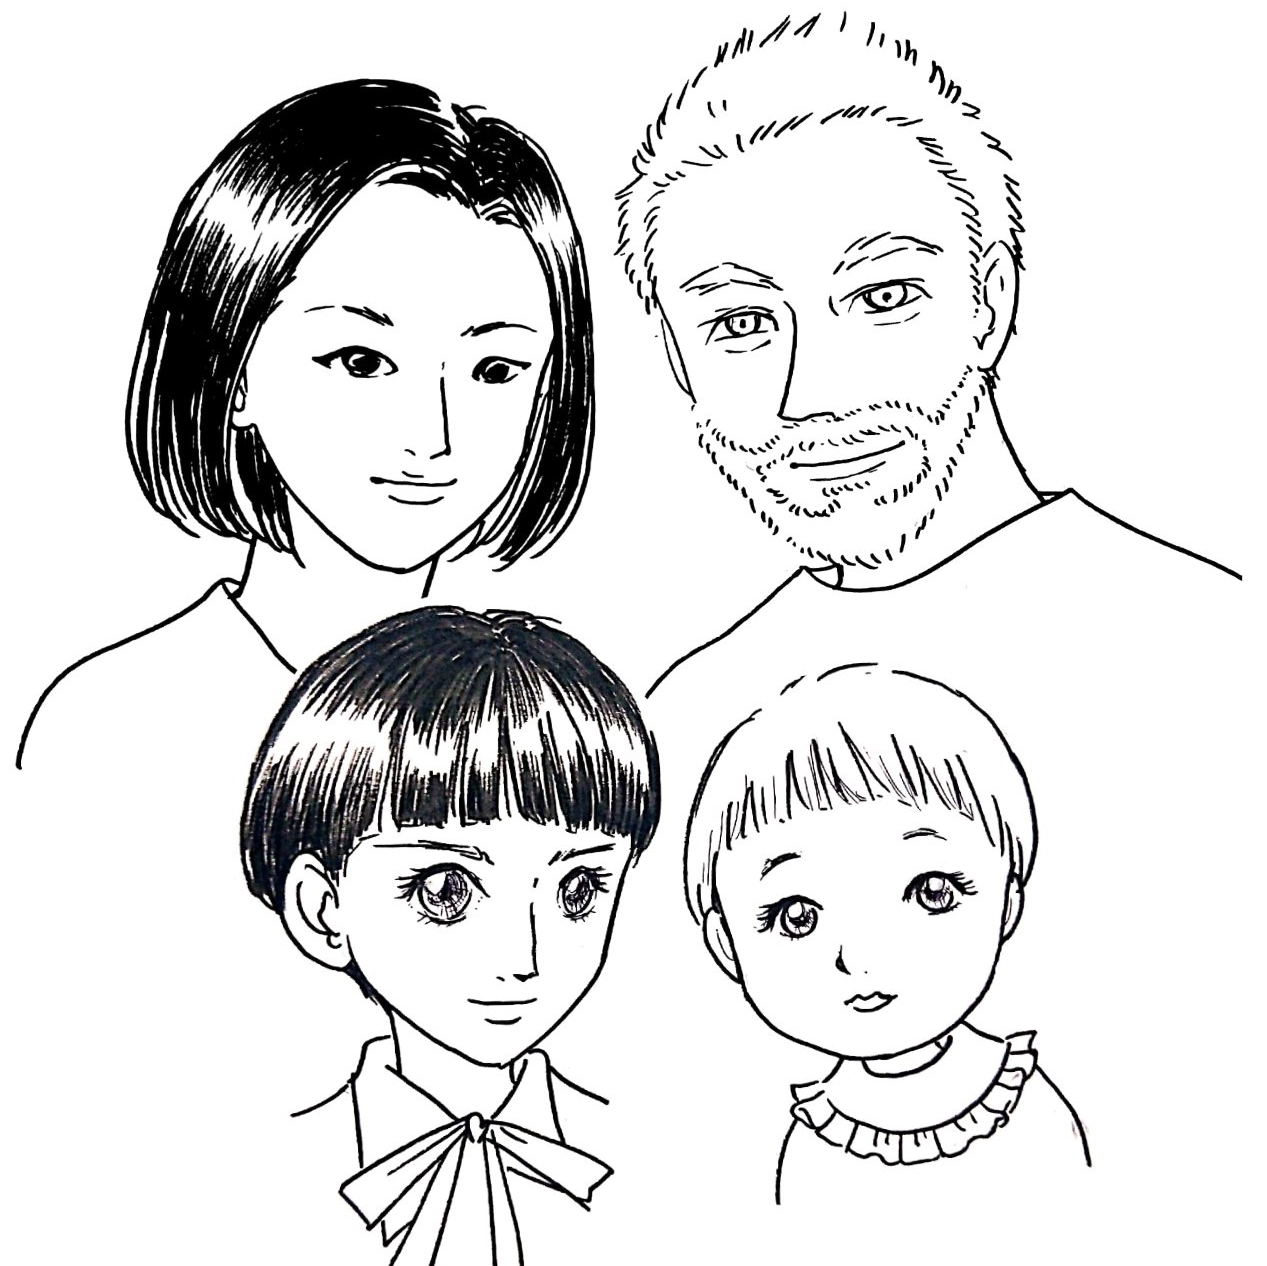
\includegraphics[width=\linewidth]{picNarrow.jpeg}
  \end{center}
  \begin{center}
      \huge \emph{{Wir suchen eine Wohnung.}}
  \end{center}
  \hrule
  \vfill
  
  \normalsize
  
\paragraph{Kontakt}
Wir freuen uns in jedem Fall über Ihre Nachricht.
\begin{itemize}
\item \url{drheindel@pm.me}
\item \texttt{+49 151 45 61 75 23}
\end{itemize}
\end{minipage}%
\quad\quad\quad
\begin{minipage}[c]{.45\linewidth}
  \large
  In kurz,  wir suchen eine Wohnung—am liebsten 2½ oder 3 Zimmer—zwischen Schöneberg und Steglitz. Da wird unser Sohn Kai nämlich zur Schule gehen. Ach so, wer sind wir eigentlich! 

\paragraph{\large Enno}
Das ist der neueste Zuwachs der Familie. 18-Monate jung, lustig, friedseelig und im Moment ganz großer Fan von `Auto` und `Wau Wau`. Enno geht auch schon zu Ingrids Kindergarten. 

\paragraph{\large Kai}
Das ist unser cleverer 5-jährige Weltenbummler, der in Kopenhagen geboren wurde und nach Abstechern nach Leipzig und Hawaii nun die Kita Buddelkiste besucht. 
Kai wird in die Rothenburg-Grundschule eingeschult werden. 

\paragraph{\large Mama}
Die Mama hat den Papa in Paris kennengelernt, während Ihres Forschungsaufenthaltes am Institut Pasteur, als promovierte Virologin. 

\paragraph{\large Papa}
Der Papa ist seit Dezember 2019 Habilitand der Informatik an der TU Berlin.

\end{minipage}

\end{document}
